\chapter{Les lentilles et les images}\label{ch:g8:lenses-images}

La chambre noire à trou d'aiguille payait sa petite \omterm{prop:g5:mirrors-reflection:image}{image} nette d'un
prix cruel~: presque pas de \omterm{def:g1:light-and-shadows:source}{lumière}. Et pourtant ton propre œil peint
tout le jour un monde lumineux et net sur sa paroi du fond, sans le
moindre trou d'aiguille en vue. Le secret de l'œil est un disque de
matière vitreuse et bombée qui recueille un \omterm{def:g6:light-propagation:ray}{faisceau} entier et le
plie à la demande --- la \omterm{def:g8:lenses-images:families}{lentille}, vedette des appareils photo, des
lunettes, des loupes et de ce chapitre.

\section{Deux familles de lentilles}

\begin{definition}[Lentilles convergentes et divergentes]\label{def:g8:lenses-images:families}
Une \emph{lentille}\index{lentille} est un morceau de matière
transparente --- verre ou plastique clair --- aux faces bombées,
construit pour dévier la \omterm{def:g1:light-and-shadows:source}{lumière} de façon contrôlée (la \omterm{def:g1:light-and-shadows:source}{lumière} est
déviée quand elle entre dans le verre~; la loi exacte de cette
déviation est un trésor du lycée). Deux familles~:
\begin{enumerate}
  \item les \emph{lentilles convergentes}\index{lentille convergente}
        --- plus épaisses au milieu qu'au bord --- rapprochent les
        rayons d'un \omterm{def:g6:light-propagation:ray}{faisceau} les uns \emph{vers} les autres~;
  \item les \emph{lentilles divergentes}\index{lentille divergente}
        --- plus minces au milieu --- les écartent.
\end{enumerate}
Passe le bout du doigt sur un verre de lunettes~: un renflement
central ou un creux central range dans sa famille toutes les
lentilles de la Terre.
\end{definition}

\begin{definition}[Foyer et distance focale]\label{def:g8:lenses-images:focus}
Envoie un \omterm{def:g6:light-propagation:ray}{faisceau} de rayons parallèles --- la \omterm{def:g1:light-and-shadows:source}{lumière} du Soleil fait
l'affaire --- à travers une \omterm{def:g8:lenses-images:families}{lentille convergente}~: les rayons déviés
se croisent tous en un point derrière elle, le
\emph{foyer}\index{foyer}. La distance de la \omterm{def:g8:lenses-images:families}{lentille} au foyer est
la \emph{distance focale}\index{distance focale} $f$~: l'unique
nombre qui définit la \omterm{def:g8:lenses-images:families}{lentille}. Les \omterm{def:g8:lenses-images:families}{lentilles} fortement bombées,
épaisses, dévient beaucoup --- $f$ court~; les \omterm{def:g8:lenses-images:families}{lentilles} à peine
bombées dévient peu --- $f$ long.
\end{definition}

\begin{omfigure}
\begin{tikzpicture}[scale=0.8]
  \draw[thick, fill=blue!6]
    (2.6,-1.6) .. controls (3.3,0) .. (2.6,1.6)
    .. controls (1.9,0) .. (2.6,-1.6);
  \foreach \y in {-1.2,-0.6,0,0.6,1.2} {
    \draw[-Stealth, omThm, thick] (0.2,\y) -- (2.35,\y);
    \draw[omThm, thick] (2.35,\y) -- (5.6,0);
  }
  \fill[omDef] (5.6,0) circle (0.09);
  \node[below, font=\small] at (5.6,-0.25) {foyer};
  \draw[Stealth-Stealth, omExo] (2.6,-1.9) -- (5.6,-1.9);
  \node[below, font=\small, omExo] at (4.1,-2.0)
    {distance focale $f$};
  \begin{scope}[xshift=7.6cm]
    \draw[thick, fill=blue!6]
      (0.95,1.6) .. controls (1.25,0.55) and (1.25,-0.55) ..
      (0.95,-1.6) -- (1.65,-1.6)
      .. controls (1.35,-0.55) and (1.35,0.55) .. (1.65,1.6)
      -- cycle;
    \foreach \y in {-1.0,-0.5,0,0.5,1.0} {
      \draw[-Stealth, omThm, thick] (0,\y) -- (0.9,\y);
      \draw[omThm, thick] (0.9,\y) -- (1.3,\y) -- (3.6,{\y*1.9});
    }
    \node[below, font=\small] at (1.8,-2.0)
      {divergente~: le faisceau s'écarte};
  \end{scope}
\end{tikzpicture}

{\small Les deux familles au travail~: la \omterm{def:g8:lenses-images:families}{lentille convergente}
rassemble un \omterm{def:g6:light-propagation:ray}{faisceau} parallèle en son \omterm{def:g8:lenses-images:focus}{foyer}~; la \omterm{def:g8:lenses-images:families}{lentille divergente}
l'ouvre en éventail.}
\end{omfigure}

\begin{method}[Mesurer une distance focale]\label{met:g8:lenses-images:measure}
Pour toute \omterm{def:g8:lenses-images:families}{lentille convergente}, une minute et une fenêtre lointaine~:
\begin{enumerate}
  \item se placer face à un mur, en vis-à-vis d'une scène
        \emph{lointaine} et lumineuse --- la fenêtre et le monde
        au-delà~;
  \item tenir la \omterm{def:g8:lenses-images:families}{lentille} près du mur et l'en éloigner lentement
        jusqu'à ce que la scène saute en une petite \omterm{prop:g5:mirrors-reflection:image}{image} nette sur
        le mur (à l'envers --- comme on s'y attend désormais)~;
  \item \omterm{def:g6:measurement-in-science:measuring}{mesurer} la distance de la \omterm{def:g8:lenses-images:families}{lentille} au mur~: pour une scène
        lointaine, cette distance \emph{est} la \omterm{def:g8:lenses-images:focus}{distance focale} ---
        les rayons venus de loin arrivent pratiquement parallèles,
        et des rayons parallèles se rassemblent au \omterm{def:g8:lenses-images:focus}{foyer}.
\end{enumerate}
Une loupe mesure autour de \qty{10}{cm}~; des verres de lunettes, des
dizaines de \omterm{def:g2:measuring-length:units}{centimètres}~; la \omterm{def:g8:lenses-images:families}{lentille} trapue d'un appareil photo,
quelques-uns.
\end{method}

\begin{remark}[La loupe qui brûle]\label{rem:g8:lenses-images:burning}
Au \omterm{def:g8:lenses-images:focus}{foyer} d'une \omterm{def:g8:lenses-images:families}{lentille convergente}, toute une largeur de \omterm{def:g6:light-propagation:ray}{faisceau} de
\omterm{def:g1:light-and-shadows:source}{lumière} solaire se tasse en un point éblouissant --- assez concentré
pour carboniser du papier et allumer un feu en quelques secondes.
Traite-la pour ce qu'elle est~: le principe du four solaire en format
de poche. Ne concentre jamais la \omterm{def:g1:light-and-shadows:source}{lumière} du Soleil près de quoi que ce
soit d'inflammable, jamais vers la peau ou les vêtements --- et, deux
fois plutôt qu'une pour la vieille loi, ne regarde jamais le Soleil
\emph{à travers} une \omterm{def:g8:lenses-images:families}{lentille}~: la mise au point de l'œil ajoutée à
celle de la \omterm{def:g8:lenses-images:families}{lentille} fait une brûlure instantanée, indolore et
définitive.
\end{remark}

\section{La lentille faiseuse d'images}

\begin{proposition}[Images réelles]\label{prop:g8:lenses-images:realimage}
Une \omterm{def:g8:lenses-images:families}{lentille convergente} recueille les rayons diffusés par chaque
point d'un objet et les livre en un point correspondant de l'autre
côté~: point par point, elle assemble une véritable \omterm{prop:g5:mirrors-reflection:image}{image} --- une
\emph{image réelle}\index{image réelle} --- qu'un écran peut
recueillir. L'\omterm{prop:g5:mirrors-reflection:image}{image} est renversée, comme celle du trou d'aiguille,
mais lumineuse~: la \omterm{def:g8:lenses-images:families}{lentille} récolte une pleine \omterm{def:g8:lenses-images:families}{lentille} de \omterm{def:g1:light-and-shadows:source}{lumière}
par point là où le trou d'aiguille n'en laissait passer qu'un fil.
Règles empiriques de la géométrie~: un objet lointain donne une \omterm{prop:g5:mirrors-reflection:image}{image}
petite et proche du \omterm{def:g8:lenses-images:focus}{foyer}~; à mesure que l'objet s'approche de la
\omterm{def:g8:lenses-images:families}{lentille}, son \omterm{prop:g5:mirrors-reflection:image}{image} recule et grandit.
\end{proposition}

\begin{omfigure}
\begin{tikzpicture}[scale=0.8]
  \draw[-Stealth, very thick, omDef] (0.8,0) -- (0.8,1.5);
  \node[left, font=\small] at (0.65,0.75) {objet};
  \draw[thick, fill=blue!6]
    (4.6,-2.0) .. controls (5.3,0) .. (4.6,2.0)
    .. controls (3.9,0) .. (4.6,-2.0);
  \draw[dashed] (0,0) -- (10.6,0);
  \draw[omThm, thick] (0.8,1.5) -- (4.6,1.5) -- (8.9,-1.13);
  \draw[omThm, thick] (0.8,1.5) -- (8.9,-1.13);
  \fill[omDef] (6.05,0) circle (0.07);
  \node[below, font=\footnotesize] at (6.05,-0.15) {foyer};
  \draw[-Stealth, very thick, omDef] (8.9,0) -- (8.9,-1.13);
  \node[right, font=\small] at (9.05,-0.6)
    {image réelle, renversée};
\end{tikzpicture}

{\small La fabrication de l'\omterm{prop:g5:mirrors-reflection:image}{image}~: les rayons issus de la pointe de
l'objet --- l'un par le centre de la \omterm{def:g8:lenses-images:families}{lentille}, l'autre dévié par le
\omterm{def:g8:lenses-images:focus}{foyer} --- se croisent de nouveau de l'autre côté, et le tableau
s'assemble là, à l'envers.}
\end{omfigure}

\begin{example}[L'appareil photo et l'œil, une seule architecture]\label{ex:g8:lenses-images:cameraeye}
Un appareil photo est la faiseuse d'\omterm{prop:g5:mirrors-reflection:image}{images} mise en boîte~: \omterm{def:g8:lenses-images:families}{lentille
convergente} devant, écran sensible à la \omterm{def:g1:light-and-shadows:source}{lumière} derrière, \omterm{prop:g5:mirrors-reflection:image}{image}
renversée formée dessus (le logiciel fait poliment pivoter le
fichier). Ton œil est la même machine en tissu vivant~: une \omterm{def:g8:lenses-images:families}{lentille
convergente} derrière la pupille, la \emph{rétine} comme écran au
fond, \omterm{prop:g5:mirrors-reflection:image}{image} renversée --- le cerveau la retourne, comme on l'avait
noté quand le trou d'aiguille nous l'apprit. La mise au point diffère
joliment~: l'appareil photo déplace sa \omterm{def:g8:lenses-images:families}{lentille}~; la \omterm{def:g8:lenses-images:families}{lentille} souple
de l'œil, elle, \emph{change de forme}, tirée plus épaisse pour le
proche, relâchée plus mince pour le lointain --- tu en sens l'effort
après une heure de lecture rapprochée.
\end{example}

\begin{example}[Les lunettes]\label{ex:g8:lenses-images:spectacles}
Quand la mise au point de l'œil ne suffit plus, une \omterm{def:g8:lenses-images:families}{lentille} placée
devant la complète. L'œil myope fait converger trop fort --- les
scènes lointaines s'assemblent \emph{avant} la rétine et arrivent
floues~: un verre \emph{divergent} défait juste ce qu'il faut de la
déviation. Les yeux hypermétropes (et la plupart des yeux âgés) font
converger trop faiblement pour le travail de près~: un verre
\emph{convergent} prête la \omterm{def:g2:pushes-and-pulls:force}{force} qui manque --- les lunettes de
lecture sont d'honnêtes petites cousines de la loupe. Deux familles
de \omterm{def:g8:lenses-images:families}{lentilles}, deux familles de flou.
\end{example}

\section{La loupe}

\begin{omfigure}
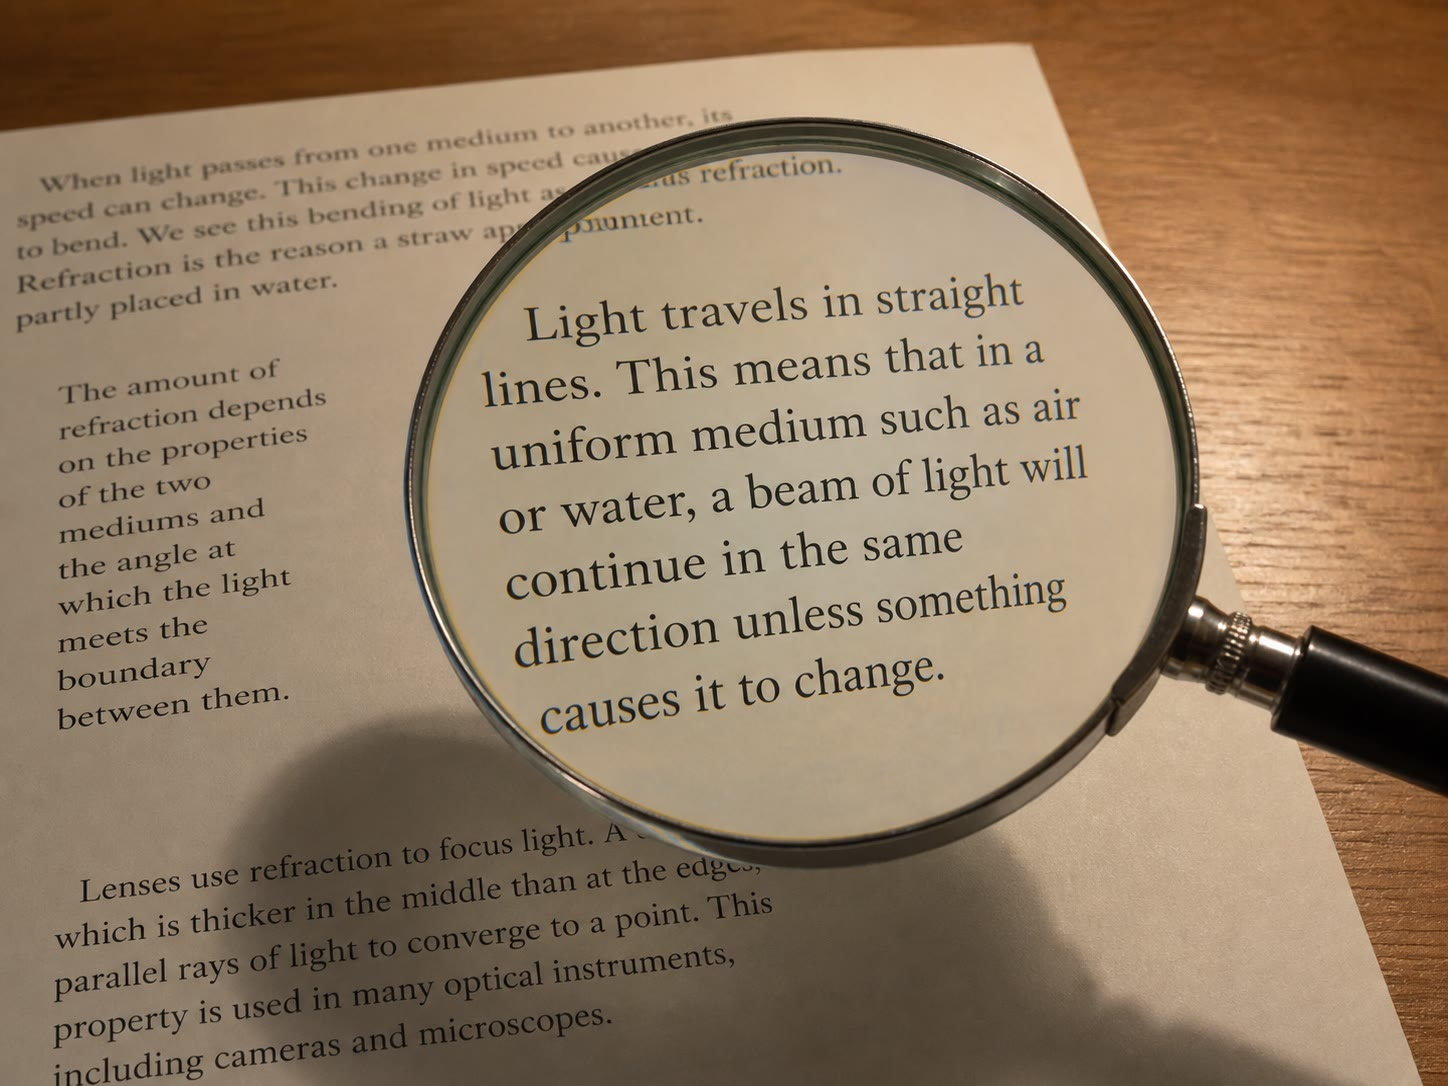
\includegraphics[width=0.5\linewidth]{images/book1/ai/g8-lenses-magnifier.jpg}

{\small La loupe au travail~: tenue plus près que sa \omterm{def:g8:lenses-images:focus}{distance focale}, la \omterm{def:g8:lenses-images:families}{lentille} montre le texte à l'endroit et agrandi.}
\end{omfigure}

\begin{example}[En deçà de la distance focale]\label{ex:g8:lenses-images:magnifier}
Tiens une \omterm{def:g8:lenses-images:families}{lentille convergente} \emph{plus près} d'un timbre que sa
\omterm{def:g8:lenses-images:focus}{distance focale}, et le tableau change de nature~: aucune \omterm{prop:g5:mirrors-reflection:image}{image} ne se
pose sur un écran --- au lieu de cela, en regardant à travers la
\omterm{def:g8:lenses-images:families}{lentille}, tu vois le timbre à l'endroit, à sa place, et agrandi. La
\omterm{def:g8:lenses-images:families}{lentille} plie les rayons du timbre de sorte qu'ils atteignent l'œil
\emph{comme s'ils} étaient diffusés par un timbre plus grand situé
derrière le verre --- une illusion sur mesure, cousine du monde
fantôme du \omterm{def:g5:mirrors-reflection:reflection}{miroir}. Les horlogers, les philatélistes et toi-même
autrefois, avec la loupe de ton enfance, l'ont tous employée~; toute
la géométrie des rayons de ce tour est un joyau du volume de lycée.
\end{example}

\begin{remark}[Des instruments sur des instruments]\label{rem:g8:lenses-images:instruments}
Empile les \omterm{def:g8:lenses-images:families}{lentilles} et le monde s'ouvre. Deux \omterm{def:g8:lenses-images:families}{lentilles convergentes}
font un microscope~: l'une jette une grande \omterm{prop:g8:lenses-images:realimage}{image réelle} d'une
gouttelette, la seconde agrandit cette \omterm{prop:g5:mirrors-reflection:image}{image} --- c'est ainsi que les
défenseurs des \omterm{def:g7:states-of-matter:molecule}{molécules} trouvèrent leurs premiers alliés directs.
Une grande \omterm{def:g8:lenses-images:families}{lentille} (ou un \omterm{def:g5:mirrors-reflection:reflection}{miroir} courbe) plus une loupe font une
lunette astronomique~: les faibles rayons parallèles de la galaxie
lointaine rassemblés en une \omterm{prop:g8:lenses-images:realimage}{image réelle}, puis agrandis jusque dans un
œil stupéfait. Tout instrument d'optique de la civilisation est fait
des deux idées de ce chapitre --- rassembler, puis agrandir --- en
diverses dispositions.
\end{remark}

\section{Exercices}

\begin{exercise}[$\star$]\label{exo:g8:lenses-images:1}
Trier au toucher~: comment le bout du doigt distingue-t-il une
\omterm{def:g8:lenses-images:families}{lentille convergente} d'une divergente~? Que fait chacune d'un \omterm{def:g6:light-propagation:ray}{faisceau}
parallèle~?
\end{exercise}

\begin{exercise}[$\star$]\label{exo:g8:lenses-images:2}
Définis le \omterm{def:g8:lenses-images:focus}{foyer} et la \omterm{def:g8:lenses-images:focus}{distance focale}. Que dit une courte \omterm{def:g8:lenses-images:focus}{distance
focale} sur la courbure d'une \omterm{def:g8:lenses-images:families}{lentille} et sur son pouvoir de
déviation~?
\end{exercise}

\begin{exercise}[$\star$]\label{exo:g8:lenses-images:3}
Décris la mesure de $f$ par la fenêtre et le mur. Pourquoi la scène
doit-elle être lointaine~?
\end{exercise}

\begin{exercise}[$\star$]\label{exo:g8:lenses-images:4}
Énonce deux règles de sécurité de la loupe qui brûle, et la raison
d'être de chacune.
\end{exercise}

\begin{exercise}[$\star$]\label{exo:g8:lenses-images:5}
Qu'est-ce qu'une \omterm{prop:g8:lenses-images:realimage}{image réelle}~? Donne ses deux propriétés
caractéristiques, et l'avantage de la \omterm{def:g8:lenses-images:families}{lentille} sur le trou
d'aiguille.
\end{exercise}

\begin{exercise}[$\star$]\label{exo:g8:lenses-images:6}
Fais correspondre l'appareil photo et l'œil~: qui joue la \omterm{def:g8:lenses-images:families}{lentille},
l'écran et le mécanisme de mise au point dans chacun~?
\end{exercise}

\begin{exercise}[$\star$]\label{exo:g8:lenses-images:7}
Quelle famille de verres sert l'œil myope, et pourquoi~? Et l'œil
hypermétrope vieillissant~?
\end{exercise}

\begin{exercise}[$\star$]\label{exo:g8:lenses-images:8}
Que doit vérifier la position du timbre pour le tour de la loupe ---
et de quelle sorte d'«~\omterm{prop:g5:mirrors-reflection:image}{image}~» l'œil jouit-il alors~?
\end{exercise}

\begin{exercise}[$\star\star$]\label{exo:g8:lenses-images:9}
Le sujet d'un photographe s'avance vers l'appareil. Dans quel sens la
\omterm{def:g8:lenses-images:families}{lentille} doit-elle bouger pour garder l'\omterm{prop:g5:mirrors-reflection:image}{image} nette sur le capteur,
d'après les règles empiriques~? Que fait l'œil, lui, dans la même
situation~?
\end{exercise}

\begin{exercise}[$\star\star$]\label{exo:g8:lenses-images:10}
Par temps ensoleillé, une \omterm{def:g8:lenses-images:families}{lentille} posée sans précaution sur des
feuilles sèches est un incendie en attente --- mais à une seule
distance lentille-feuille bien précise. Laquelle, et pourquoi
exactement là~?
\end{exercise}

\begin{exercise}[$\star\star$]\label{exo:g8:lenses-images:11}
Les lunettes de lecture du grand-père servent aussi de loupe de
secours et, les jours de vacances, d'allume-cigare solaire --- mais
celles de son petit-fils myope ne font ni l'un ni l'autre. Explique
les deux faits de famille.
\end{exercise}

\begin{exercise}[$\star\star\star$]\label{exo:g8:lenses-images:12}
Le microscope et la lunette astronomique empilent tous deux deux
\omterm{def:g8:lenses-images:families}{lentilles convergentes} --- et pourtant l'un grossit des gouttelettes
et l'autre des galaxies. Oppose leurs deux étages~: que reçoit et que
produit la \omterm{def:g8:lenses-images:families}{lentille} numéro un dans chaque instrument (objet proche
contre \omterm{def:g1:light-and-shadows:source}{lumière} d'\omterm{def:g4:solar-system:star}{étoile} pratiquement parallèle), et pourquoi la
lunette veut-elle avant tout une \omterm{def:g8:lenses-images:families}{lentille} numéro un \emph{grande},
tandis que le microscope la veut \emph{fortement bombée}~?
\end{exercise}

\section{Problème~: l'établi de l'opticien}

\begin{problem}[{Problème du week-end --- en apprentissage chez
l'opticien du bourg~; des distances focales, des équipements et une
lunette fêlée}]\label{pb:g8:lenses-images:1}
Une journée chez l'opticien~: des \omterm{def:g8:lenses-images:families}{lentilles} à trier, des lunettes à
accorder, et la lunette astronomique d'un client en pièces
détachées.

\medskip\noindent\textbf{Partie I --- trier le plateau.}
Un tiroir renversé a mélangé le stock.
\begin{enumerate}
  \item Propose deux essais rapides --- un au toucher, un avec la
        fenêtre et le mur --- pour séparer les \omterm{def:g8:lenses-images:families}{lentilles
        convergentes} des divergentes.
  \item La \omterm{def:g8:lenses-images:families}{lentille} A jette une \omterm{prop:g5:mirrors-reflection:image}{image} nette de la rue sur le mur à
        \qty{25}{cm}. Sa \omterm{def:g8:lenses-images:focus}{distance focale} et sa famille~?
  \item La \omterm{def:g8:lenses-images:families}{lentille} B refuse de jeter la moindre \omterm{prop:g5:mirrors-reflection:image}{image} sur le mur à
        quelque distance que ce soit, et les objets vus à travers
        elle paraissent plus petits. Sa famille~?
  \item Les \omterm{def:g8:lenses-images:families}{lentilles} C et D sont toutes deux convergentes~; C fait
        son \omterm{prop:g5:mirrors-reflection:image}{image} de la fenêtre à \qty{10}{cm}, D à \qty{40}{cm}.
        Laquelle est la plus bombée, celle qui dévie le plus fort~?
\end{enumerate}

\medskip\noindent\textbf{Partie II --- les équipements.}
\begin{enumerate}[resume]
  \item Un client voit flous les panneaux de route lointains mais
        lit les menus sans effort. Diagnostique l'œil et prescris
        la famille.
  \item Un autre tient son journal à bout de bras et se plaint que
        ses bras sont «~trop courts~». Diagnostique et prescris.
  \item L'opticien avertit le second client~: «~vos nouvelles
        lunettes de lecture rendront les montagnes floues.~»
        Pourquoi les lunettes de lecture ne valent-elles que pour
        les pages proches~?
  \item Un enfant demande pourquoi les verres d'essai de l'opticien
        font tanguer l'échelle de lecture alors que ses propres
        yeux vont «~très bien~». Que fait un verre correcteur à un
        œil déjà bien accommodé~?
\end{enumerate}

\medskip\noindent\textbf{Partie III --- la lunette fêlée.}
Un client apporte une lunette d'observation des \omterm{def:g4:solar-system:star}{étoiles} dont la
\omterm{def:g8:lenses-images:families}{lentille} de devant est fêlée, et demande si la loupe de rechange
rangée dans la boîte peut la remplacer.
\begin{enumerate}[resume]
  \item Nomme les tâches des deux \omterm{def:g8:lenses-images:families}{lentilles} dans l'instrument en bon
        état~: que reçoit la grande \omterm{def:g8:lenses-images:families}{lentille} de devant d'une \omterm{def:g4:solar-system:star}{étoile}
        et qu'en fait-elle, et que fait de cela la petite \omterm{def:g8:lenses-images:families}{lentille}
        d'œil~?
  \item La \omterm{def:g8:lenses-images:families}{lentille} de devant est large comme une soucoupe~; la
        \omterm{def:g8:lenses-images:families}{lentille} d'œil, grande comme une pièce de monnaie. Pourquoi
        la \emph{largeur} de la \omterm{def:g8:lenses-images:families}{lentille} de devant compte-t-elle
        tant pour les \omterm{def:g4:solar-system:star}{étoiles} faibles~?
  \item La loupe de rechange est fortement bombée mais grande comme
        une pièce de monnaie. Juge le remplacement~: que
        gagnerait-on et que perdrait-on à l'avant de l'instrument~?
  \item Clos la journée par le credo de l'opticien en une ligne sur
        tous les instruments de l'étagère --- lunettes, loupes,
        appareils photo, lunettes astronomiques --- et le résumé en
        deux verbes de ce que les \omterm{def:g8:lenses-images:families}{lentilles} font pour la
        civilisation.
\end{enumerate}
\end{problem}
